\section{Real Domain tests}
\label{sec:realDomainTests}
	In order to have a better idea of the quality of the methods previously show I tested them with real instance. These instances are taken from the gerber files avaible from the following online archive:
	\begin{itemize}
		\item \href{https://www.maximintegrated.com/en/design/tools/cad-layout/gerber/}{https://www.maximintegrated.com/en/design/tools/cad-layout/gerber/};
		\item \href{https://www.microchip.com/doclisting/TechDoc.aspx?type=Gerber}{https://www.microchip.com/doclisting/TechDoc.aspx?type=Gerber} ;
	\end{itemize}

	I explored a dozens of project and select some drill gerber files, from these I made\footnote{This could be done thank to the parser developed by my colleagues Sebastiano Valle and Mirko Bez.} the following \verb|.dat|:
	
	\begin{itemize}
		\item \verb|SC_545|
		\item \verb|MAX_682|
		\item \verb|DS_1120|
	\end{itemize}
	Figure~\ref{fig:SC_545} shows a representation of one of them. The other could be seen from the pdf inside the \verb|RealInstances| folder attached to this report.

	\begin{figure}
		\centering
		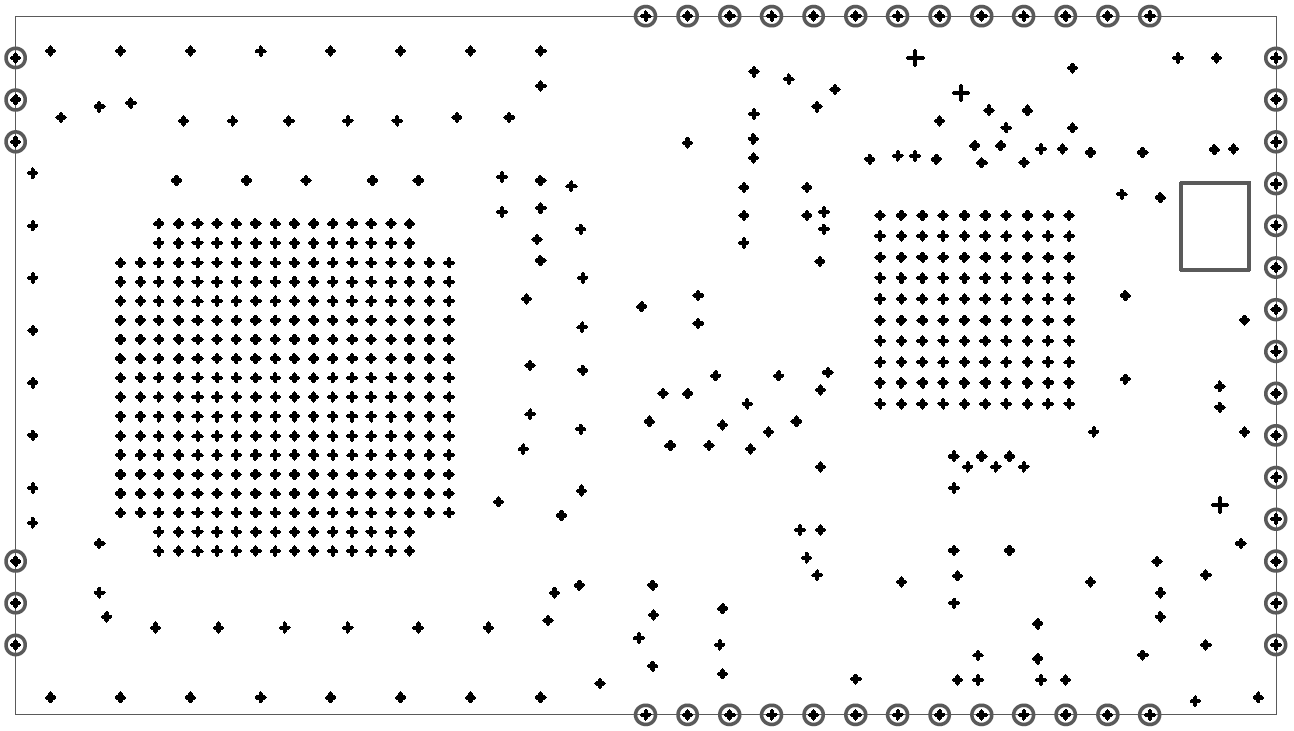
\includegraphics[width=\textwidth]{img/SC_545}
		\caption{The representation of the SC\_545 real instance.}
		\label{fig:SC_545}
	\end{figure}
	
	
	
	\subsection{Results exact method}
		The instances are too huge and the power of computation is too low in order to test the exact method implemented with CPLEX in an amount of time for this project purpose. Neither with a timeout the CPLEX API can give me a intermediate solution in a reasonable amount of time.
		
	\newpage
	
	\subsection{Results Local Search}
	
	
	
		
		
	